\chapter{Grundlagen}
\label{chap:grundlagen}
Im Folgenden gibt es eine Erläuterung und Erklärung der technischen Grundlagen, dies umfasst die beiden zentralen, verwenden Konzepten, das Aloha Protokoll und das Stromnetz sowie auch eine Einführung zu Elektrofahrzeugen.

\section{Aloha-Protokoll}
\label{capBack:Aloha}
Das Aloha Protokoll wurde an der Universität von Hawaii entwickelt \cite{aloha_firstsource}. Ursprünglich wurde es dort für Übertragungen zwischen Funkstationen entwickelt, allerdings lässt sich das Protokoll überall dort verwenden, wo unkoordinierte Benutzer mit einem geteilten Medium arbeiten \cite{Back_AlohaPure}. Das Aloha Netzwerkprotokoll definiert wie alle Protokolle Regeln und Formate, welche den Ablauf der Kommunikation bestimmen. In der heutigen Form des Internets bzw der Kommunikation über ein Netzwerk, arbeiten mehrere verschiedene Protokolle, welche sich jeweils mit verschiedenen Schritten befassen und unterschiedliche Aufgaben erfüllen, zusammen. Diese Zusammenarbeit lässt sich für die Netzwerkkommunikation über das ISO/OSI Schichtenmodell erläutern. Der Weg der Daten von der vom Nutzer verwendeten Anwendung bis zur eigentlichen Aktivität auf einer Leitung eines Netzwerkes wird in sieben Schritte eingeteilt. Die Reihenfolge dieser Schritte beim Senden von Daten ist genau gegensätzlich zu der Reihenfolge beim Empfangen von Daten. Jede Schicht hat dabei ihre spezielle Aufgabe, was sie von den anderen Schichten abgrenzt. Beim Senden von Daten durchläuft man die Schichten in folgender Reihenfolge, Anwendungsschicht, Dartstellungsschicht, Sitzungsschicht, Transportschicht, Vermittlungsschicht, Sicherungsschicht und Übertragungsschicht. Das Aloha Protokoll arbeitet auf der Sicherungsschicht, auf dieser Ebene soll ein Protokoll in der Lage sein eine fehlerfreie Übertragung zu ermöglichen und den Zugriff auf das Übertragungsmedium zu regeln. Die Daten, welche mithilfe des Aloha Protokolls versendet werden sollen, werden in Frames eingeteilt. In einem solchen Frame werden die Daten in zwei Bereiche unterteilt. Der erste Teil der Daten wird vom Aloha Protokoll selbst benötigt, für die Weiterleitung der Daten, dies ist auch der Teil eines Frames, welcher vom Aloha Protokoll generiert bzw. verarbeitet wird. Der zweite Teil der Daten enthält den eigentlichen Inhalt des Frames, welcher versendet oder empfangen werden soll. Der zweite Teil enthält Daten welche vom Aloha Protokoll nicht verarbeitet, sondern nur weitergegeben werden sollen. Das Medium bzw. das Netzwerk über welches das Aloha Protokoll Frames empfangen oder versenden soll muss immer mit allen Teilnehmern geteilt werden. Jeder Teilnehmer ist über das passive Übertragungsmedium mit allen anderen Teilnehmern verbunden. Das passive Übertragungsmedium kann allerdings nur von einem Teilnehmer gleichzeitig genutzt werden, also kann nur ein Frame gleichzeitig übertragen werden. Die Tatsache, dass immer nur ein Paket gleichzeitig übertragen werden kann, ist für das Aloha Protokoll ein nicht vernachlässigbarer Nachteil. Die Teilnehmer agieren bei der Verwendung des Protokolls unabhängig voneinander und prüfen vor Beginn einer Datenübertragung nicht die aktuelle Aktivität auf dem Übertragungsmedium. Diese fehlende Überprüfung auf Aktivität auf dem Übertragungsmedium bedeutet, dass das Aloha Protokoll nicht carrier sensitiv ist. Das unabhängige Agieren voneinander hat zur Folge, dass eine Datenübertragung zu jedem beliebigen Zeitpunkt beginnen kann. Die Kombination von drei Eigenschaften trägt stark zur Minderung der möglichen Effizienz bei. Diese Eigenschaften sind die beliebigen Wahl eines Startzeitpunktes für eine Übertragung, die fehlenden Überprüfung von bereits vorherrschender Aktivität und die Tatsache, das nur ein einzelner Frame gleichzeitig übertragen werden kann. Durch diese Eigenschaften sinkt die Effizenz so weit ab, dass nur etwa 18.4\% der Zeit für erfolgreiche Übertragungen genutzt werden können \cite{Back_AlohaPure}. In der restlichen Zeit treten Kollisionen auf, gesendete Daten werden nicht erfolgreich übertragen \cite{Back_AlohaPure}. Im Zusammenhang mit dem Aloha Protokoll bezeichnet eine Kollision einen fehlgeschlagenen Versuch einen Frame zu übertragen. Eine Kollision tritt also immer dann auf, wenn mehrere Teilnehmer gleichzeitig versuchen einen Frame zu übertragen. Diese Frames können nicht mehr voneinander unterschieden werden und sind deshalb für die anderen Teilnehmer nicht verständlich. Nach dem Auftreten einer Kollision wird ein zuvor kollidierter Frame allerdings nicht sofort wieder gesendet. Vor einem erneuten Versuch den Frame zu übertragen wartet der Teilnehmer eine gewisse Zeit, welche zufällig bestimmt wird. Durch die zufällige Wahl der Wartezeiten sollen verschieden lang Wartezeit erreicht werden. Durch die verschieden Längen der Wartezeiten versuchen Teilnehmer zu unterschiedlichen Zeiten erneut ihren Frame zu senden und so durch die Unterschiedlichkeit der Zeitpunkte insgesamt alle Frames erfolgreich zu übertragen.
\begin{figure}[h!]
	\begin{center}
	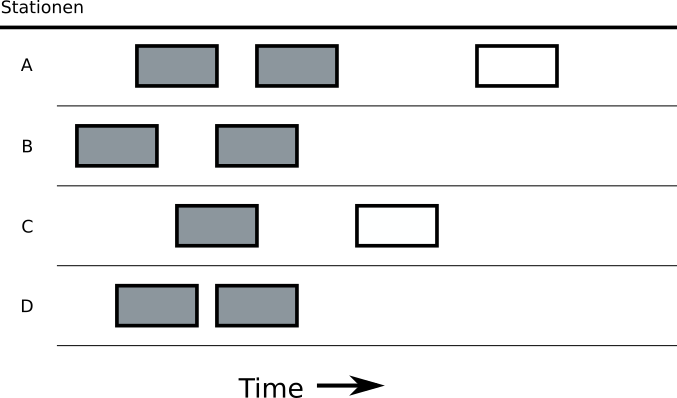
\includegraphics[scale=0.6]{img/ZeichnungExport2.png}
	\caption{Datenübertragung mit Kollisionen unter Verwendung des Aloha Protokolls}
	\end{center}
	\label{Abb2_PureAloha}
\end{figure}

In der Abbildung \ref{Abb2_PureAloha} sind insgesamt neun Kästchen, sieben in grau und zwei in weiß, aufgeteilt auf die horizontalen Kanäle A bis D entlang einer unbeschrifteten Zeitachse verteilt. In den Kanälen A bis D ist jeweils die Aktivität eines einzelnen Teilnehmers enthalten. Jedes der abgebildeten Kästchen steht für eine Frame. An den auf verschiedenen Höhen der Zeitachse gelegenen Anfängen der Frames ist die Beliebigkeit des Starts einer Übertragung erkennbar. Die grau dargestellten Kästchen stehen für Frames, welche mit anderen Frames kollidiert sind. Jedes in grau dargestellte Kästchen überschneidet sich mit einem anderem in grau dargestellten Kästchen. Jedes weiße Kästchen überschneit sich mit keinem anderem Paket, ist folglich nicht kollidiert und wurde erfolgreich übertragen.\\
Eine Weiterentwicklung des Aloha Protokolls nimmt an einigen Stellen Verbesserungen vor. Diese Weiterentwicklung nennt sich Slotted Aloha \cite{Back_AlohaPure}. Die Zeit wird in feste Abschnitte eingeteilt, wobei ein Zeitabschnitt der Übertragungsdauer eines Frames entspricht. Der Beginn eines solchen Abschnittes sind auch die Zeitpunkte an denen mit der Übertragung begonnen werden kann. Durch die Festlegung von solchen Zeitpunkten wird eine Kollision schneller entdeckt und es werden weniger Daten übertragen, welche kollidieren. Wird zu beginn der Übertragung keine Kollision festgestellt, wird dies auch nicht am Ende festgestellt. Durch diese Verbesserung wurde der Anteil der Zeit, in der erfolgreich Daten übertragen werden, auf etwa 36.8\% erhöht, ist also etwa doppelt so hoch wie beim herkömmlichen Aloha. \cite{Back_AlohaPure}. Allerdings gilt es zu beachten, das diese gesteigerte Effizenz nur durch eine gemeinsame, synchrone Uhr erreicht werden kann.\\
\begin{figure}[h!]
	\begin{center}
	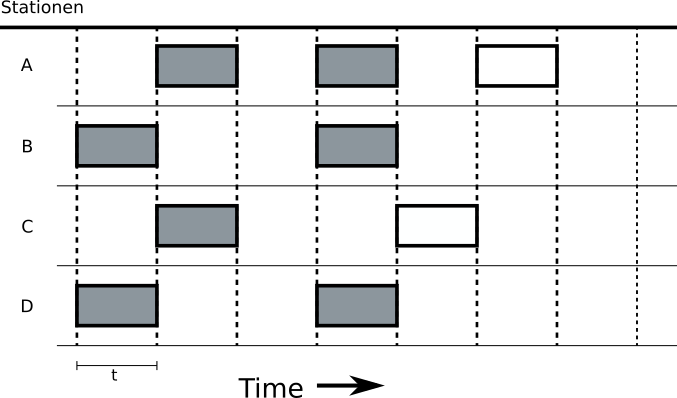
\includegraphics[scale=0.6]{img/ZeichnungExportSlotted3.png}
	\caption{Datenübertragung mit Kollisionen unter Verwendung des Slotted Aloha Protokolls}
	\end{center}
	\label{Abb_SlottedAloha}
\end{figure}
In der Abbildung \ref{Abb_SlottedAloha} sind insgesamt neun Kästchen, sieben in grau und zwei in weiß, aufgeteilt auf die horizontalen Kanäle A bis D entlang einer Zeitachse verteilt. Die Zeitachse ist in Abschnitte eingeteilt, welche durch vertikale gestrichelte Linien markiert sind. Die Abschnitte sind t Zeiteinheiten lang. Die Menge der Zeiteinheiten pro Abschnitt entspricht der Menge an Zeiteinheiten, welche nötig sind um eine Frame komplett zu übertragen. In den Kanälen A bis D ist jeweils die Aktivität eines einzelnen Teilnehmers enthalten. Jedes der abgebildeten Kästchen steht für eine Frame. Bei allen grau dargestellten Kästchen befindet sich mindestens ein weiteres Kästchen im selben Zeitabschnitt, diese Frames sind also miteinander kollidiert. Die beiden in weiß dargestellten Kästchen stehen für Frames, welche erfolgreich übertragen wurden. In den beiden Zeitabschnitten in denen sich die beiden weißen Kästchen befinden ist auch kein anderes Kästchen dargestellt, somit wurde auch nicht versucht mehr als ein Kästchen gleichzeitig zu übertragen.

\section{Elektrischer Strom}
Elektrischer Strom, Elektrizität oder umgangssprachlich auch Strom, all diese Begriffe bezeichnen die Bewegung geladener Teilchen entlang eines Leiters. Die geladen, sich bewegenden Teilchen sind gemäß geltenden physikalischen Gesetzen der Elektronenstromrichtung, in einem geschlossenen Stromkreis negativ geladen, es handelt sich also um Elektronen. Für eine erfolgreiche Übertragung von elektrischem Strom müssen genug dieser geladen Teilchen, mit der jeweils gleichen Ladung, vorhanden sein. Die Übertragung der geladenen Teilchen erfolgt über ein Medium welche genug dieser Ladungsträger verfügbar hat, ein solches Medium wird auch als Leiter bezeichnet.\\
Der elektrische Strom wird von vier Faktoren definiert, der Spannung U, der Stromstärke I, dem Widerstand R und der Leistung P. Die Spannung U, wird in der Einheit Volt (V) angegeben. Die Spannung gibt an welche Kraft auf die beweglichen Ladungsträger wirkt, je größer die Spannung, desto stärker bewegenden sich die Ladungsträger \cite{spannung_1}. Die Stromstärke wird in Ampere (A) angegeben und gibt an, wie viele Ladungsträger in einer Zeiteinheit durch einen Leiter fließen \cite{stromstaerke_1}. Je höher die Stromstärke, desto mehr Ladungsträger fließen durch den Leiter. Der Widerstand angegeben in R, gibt an wie sehr die geladen Teilchen bei ihrem Fluss durch den Leiter gestört werden \cite{widerstand_1}. Die Leistung P wird angegeben in Watt (W) und gibt an wie viel Energie/ Leistung übertragen wurde. Diese vier Faktoren sind untereinander so mit einander verbunden, dass mit der Formel \ref{strom_formel_1}, sowie ihren mathematischen Transformationen, die Spannung, die Stromstärke und der Widerstand in Verhältnis gesetzt werden können.
\begin{align}
	U  =  R \cdot I
	\label{strom_formel_1}
\end{align}
Die elektrische Leistung P wird berechnet durch die Formel \ref{strom_formel_2}.
\begin{align}
	P = U \cdot I
	\label{strom_formel_2}
\end{align}
Durch einsetzen von Formel \ref{strom_formel_1} in Formel \ref{strom_formel_2} kann P mit jeder Kombination von Spannung, Stromstärke und Widerstand bestimmt werden.\\
Die Spannung kann im Leiter auf verschiedene Arten vorliegen, in Form von Gleichspannung oder Wechselspannung. Gleichspannung fließt mit immer gleicher Stärke und immer gleicher Richtung durch den Leiter. Im Falle der Wechselspannung wechselt sowohl die Stärke, als auch die Flussrichtung in periodischen Abständen. Der Verlauf der Spannung während eines Wechselvorgangs kann verschiedene Formen annehmen, abgebildet auf Kurven kann ein rechteckiger, ein gezahnter, ein dreieckiger oder ein sinusförmiger Verlauf entstehen. Der im Stromnetz verwendet Wechsel entspricht einem sinusförmigen Verlauf. Der Widerstand hängt mit am stärksten vom verwendeten Leiter ab, je besser der Leiter geeignet ist, desto geringer ist der Widerstand. Der Widerstand eines Leiters ist auch von der Länge des Leiters abhängig, je länger ein Leiter ist, desto größer ist sein Widerstand. Bei der elektrischen Leistung muss zwischen der Wirkleistung \ref{strom_formel_2} und der Blindleistung unterschieden werden \cite{strom_leistung}. Wirk- und Blindleistung bilden zusammen die Scheinleistung. Die Wirkleistung, angegeben in Watt (W), bezeichnet den Teil der elektrischen Leistung, welcher effektiv genutzt werden kann. Die Blindleistung, angegeben mit der Einheit VAr, bezeichnet den Teil welcher zwar ins Netz eingespeist werden muss aber nicht von seinen Nutzern verbraucht werden kann. Blindleistung entsteht wenn sich die Schwingungen der Wechselspannung verschieben. Diese Verschiebung entsteht wenn elektrische Energie verschoben zur eigentlichen Schwingung wieder ins Netz eingespeist wird. Die Scheinleistung, angegeben in VA, bezeichnet nun also die Summe von Wirk- und Blindleistung also alle Leistung, welche ins Netz verfügbar ist. Der Wert der Scheinleistung kann aus den Werten für Wirk- und Blindleistung mithilfe der Formel
\begin{align}
	S = \sqrt{P^{2}+Q^{2}}
	\label{strom_formel_3}
\end{align}
berechnet werden.

\section{Aufbau des Stromnetz}
\label{capBack:Stromnetz}
Bei dem deutschen Stromnetz handelt es sich um ein Wechselspannungsnetz mit einer Normfrequenz von 50 Hz. Das Stromnetz lässt sich in zwei Ebenen einteilen, das Übertragungsnetz und das Verteilnetz. Das Übertragungsnetz ist ausgelegt auf die Übertragung von elektrischer Leistung über weite Strecken. Das Übertragungsnetz ist auch als Höchstspannungsnetz bekannt. Dies rührt daher, dass die Spannung im Übertragungsnetz höher ist als im Verteilnetz. Die Spannung ist höher, da die Transportverluste bei höheren Wechselspannungen geringer ausfallen als bei niedrigeren. Je mehr Verluste bereits beim Transport auftreten, desto mehr Leistung muss anfänglich bereitgestellt werden um dieselbe Leistung zum Abnehmer zu transportieren. Diese Abnehmer sind zu großen Teilen mit dem Verteilnetz verbunden. Im Verteilnetz herrscht aber eine andere Spannung als im Übertragungsnetz. Diese verschiedenen Spannungen können mithilfe eines Transformators ineinander umgewandelt werden. Die Bauteile dieser Transformatoren limitieren die maximale Menge an leistung welche transformiert werden kann. Einzelne Verbraucher sind auch direkt ans Übertragungsnetz angeschlossen, aufgrund ihres hohen Leistungsbedarfs. Diese Großverbraucher verfügen über eigene Transformatoren.
\begin{figure}[h!]
	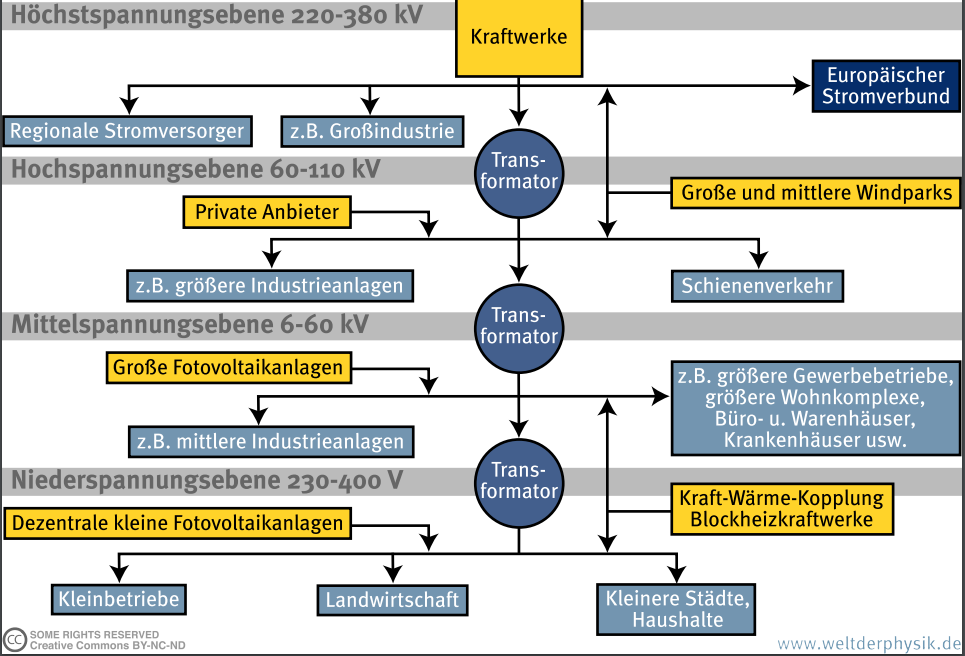
\includegraphics[width=\linewidth]{img/Stromnetz1.png}
	\caption{Aufbau des Stromnetzes}
	\label{Abb1_Stromnetz}
\end{figure}


In der Abbildung \ref{Abb1_Stromnetz} sind die verschieden Spannungsebenen des Stromnetzes aufgezeichnet. Auf den verschieden Ebenen sind verschiedene Akteure aktiv. Die gelb dargestellten Teilnehmer speisen die von Ihnen erzeugte Energie ins Stromnetz ein. Transformatoren, dargestellt als Kreise, verbinden die Spannungsebenen miteinander. Die blau dargestellten Kästchen beziehen Leistung aus dem Netz. Verbraucher auf verschiedenen Ebene des Netzes können auch verschieden große Mengen an Energie beziehen. Energieerzeuger speisen ebenfalls abhängig ihrer Leistungsfähigkeit auf verschieden Ebene des Netzes ein. Das Verteilnetz umfasst meist nur Mittel und Niederspannungsebene und manchmal auch die Hochspannungsebene. Im Zuge dieser Arbeit wird nur die Niederspannungsebene oder das Niederspannungsnetz genauer betrachtet. Ein Niederspannungsnetz verfügt im Normalfall über nur einen Transformator, welcher die elektrische Leistung für alle Abnehmer bereitstellt. Ein Niederspannungsnetz in Deutschland kann als Strahlen-, Ring- oder Maschennetz betrieben werden. Ring- und Maschennetze bieten eine höhere Versorgungsicherheit, allerdings sind Strahlennetze kostengünstiger zu realisieren. Strahlennetze sind außerdem leichter wartbar, da sich Fehlerfälle oft auf einzelne Stahlen beschränken lassen. Daher wird in dieser Arbeit im folgenden bei einem Niederspannungsnetz von einer Strahlennetz ausgegangen. Bei einem Strahlennetz sind ein oder mehr Kabelstränge mit dem Transformator verbunden. An jedem dieser Stränge sind ein oder mehrere Abnehmer verbunden. Zwischen den vom Transformator abgehenden Strängen bestehen keinerlei Verbindungen, um keine Ringschlüsse zu schaffen. Dadurch ist die Fluss Richtung des elektrischen Stroms vom Transformator zum Verbraucher immer gleich. Ein Strahlennetz bietet den Vorteil einer einfachen Planung. Im Falle einer Störung an einem oder mehreren der Strahlen, sind alle mit diesen Strahl verbunden Abnehmern betroffen.\\
Die Höhe, der im Niederspannungsnetz übertragenen, Spannung beträgt gemäß Norm (DIN EN 50160) 230V. Das Niederspannungsnetz ist in Deutschland dreiphasig konzipiert, jede der drei Phasen transportiert eine Spannung von 230V. Die Wechselspannungskurven dieser drei Phasen sind um jeweils 120 Grad zueinander verschoben. Diese Phasen sind Teil des Strahls bzw. des Kabels, welcher den Teilnehmer mit dem Transformator verbindet. Durch die Aufteilung auf drei stromführende Phasen kann mehr Leistung übertragen werden, da so mehr als eine Phase  gleichzeitig genutzt werden kann und die jeweils bezogene Mengen an Leistung aufsummiert werden. Durch Verschiebung der sinusförmigen Schwingungen des Wechselstroms (\cite{strom_phasen}) zueinander sind nur zwei der drei stromführenden Phasen gleichzeitig nutzbar. Bei Nutzung von mehr als einer Phase erhöht sich auch die verfügbare Spannung aufgrund der Verschiebung von 230 V auf 400 V statt auf 460V, dadurch sind bei gleicher Stromstärke höhere Lasten möglich.



\section{Elektrofahrzeugen}
Ein Fahrzeug kann dann als Elektrofahrzeug bezeichnet werden, wenn es in der Lage ist elektrische Energie für seine unmittelbare Fortbewegung zu nutzen. Dieses Nutzen kann auf mehrere Arten erreicht werden. Als erste zu nennen ist das batterieelektrische Fahrzeug oder Battery Electric Vehicle (BEV), bei dieser Art der Bauweise dient ein Akku als Energiespeicher für einen oder mehre Elektromotoren \cite{e_auto}. Die elektrische Energie, welche für den Betrieb des Fahrzeuges verwendet werden kann,  wird in einem Akku gespeichert. Dieser Akku wird entweder durch Rekuperation, also durch Rückumwandlung von Fortbewegungsenergie in elektrische Energie, oder durch einen Ladevorgang an einem Ladegerät geladen. Eine andere Art eines Batterie-elektrischen Fahrzeuges ist, ein batterie-elektrisches Fahrzeug mit Range-Extender \cite{e_auto}. Bei diesen kann der Akku auch mithilfe eines, im Fahrzeug verbauten, Verbrennungsmotors geladen werden. Dieser Verbrennungsmotor treibt einen Generator an, wodurch elektrischer Strom erzeugt wird, welcher dann in der Batterie gespeichert werden kann. Der Verbrennungsmotor ist aber nicht in der Lage das Fahrzeug direkt anzutreiben, wie bei der klassischen Verwendung des Verbrenners in einem Fahrzeug. Der Verbrennungsmotor ist des weiteren nicht in der Lage die volle Leistung der verbauten Elektromotoren zu bedienen. Bei leerem Akku ist die Leistung des Fahrzeuges limitiert durch die Leistung des Verbrenners. \\
Neben dem Konzept des batterie-elektrischen Antriebes gibt auch Hybride Ansätze, wo die Leistung eines Verbrenners und einem oder mehrere Elektromotoren kombiniert wird. Diese Ansätze lassen in drei Gruppen unterteilen. Bei der ersten Gruppe \cite{e_auto}, generiert ein Verbrenner mit einem Generator oder eine Brennstoffzelle, die elektrische Energie, welche der Elektromotor für den Antrieb benötigt. Der verbaute Akku dient nur zum speichern für kurze Zeit und kann nicht von außen geladen werden. In der zweiten Gruppe \cite{e_auto}, dienen die oder der verbaute Elektromotor nur zur Unterstützung des Verbrenners, nicht allerdings zum alleinigen Antrieb des Fahrzeugs. Die verbaute Batterie hat hier ebenfalls keine hohe Kapazität und kann nicht von außen geladen werden. Die dritte Gruppe beinhalten nun Systeme, welche als Hybrid Electric Vehicle (HEV) oder Plug-In Hybrid Electric Vehicle (PHEV) bekannt sind \cite{e_auto}. In beiden Fahrzeugtypen ist ein Verbrennungsmotor und einer oder mehrere Elektromotoren verbaut. Anders als bisher sind hier aber beide Motorarten jeweils alleine in der Lage das Fahrzeug zu betreiben. Fahrzeuge dieser Kategorie können wie ein herkömmlicher Verbrenner oder wie ein BEV verwendet werden. Das Merkmal was ein PHEV von einem HEV unterscheidet ist, dass bei einem PHEV die verbaute Batterie von außen über ein Ladegerät geladen werden kann. Die Ladung über einen, vom Verbrennungsmotor angetriebenen, Generator oder über Rekuperation ist hingegen sowohl beim HEV als auch beim PHEV möglich.\\
\begin{figure}[htb]
	\centering
	\begin{minipage}[t]{0.45\linewidth}
		\centering
        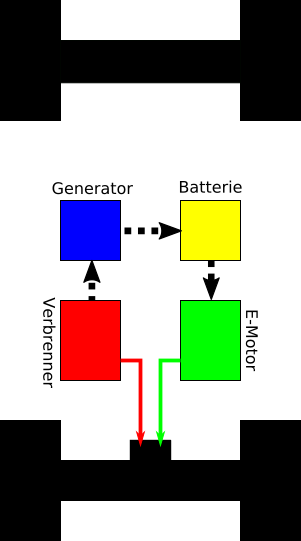
\includegraphics[width=0.8\linewidth]{img/HEV3.png}
        \caption{Hybridfahrzeug}
        \label{HEV}
	\end{minipage}
	\hfill
	\begin{minipage}[t]{0.45\linewidth}
		\centering
        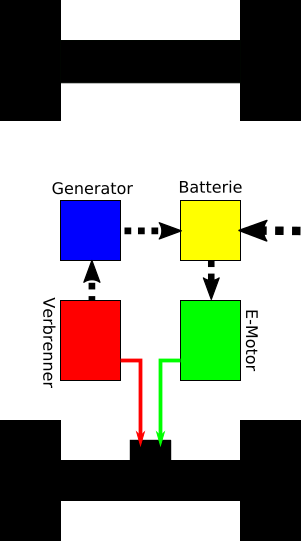
\includegraphics[width=0.8\linewidth]{img/PHEV3.png}
        \caption{Plug-In \newline Hybridfahrzeug}
        \label{PHEV}
	\end{minipage}
\end{figure}

In der Abbildung \ref{HEV} ist der schematische Aufbau eines Hybrid Fahrzeuges dargestellt. Sowohl der Verbrennungsmotor als auch der Elektromotor sind in der Lage das Fahrzeug zu betreiben. Der Weg der Energie vom Verbrennungsmotor zur Batterie über den Generator wird verdeutlicht. In der Abbildung \ref{PHEV} wird der Unterschied zwischen einem HEV und einem PHEV verdeutlicht. Beim Plug-In Hybrid ist es möglich die Batterie des Fahrzeugs von außen über ein Ladegerät zu laden.\\
Innerhalb dieser Arbeit werden jene Arten von Elektrofahrzeugen betrachtet, deren Batterie mithilfe eines Ladegerätes geladen werden kann. Zu dieser Art zählen die Battery Electric Vehicles (BEV), BEV mit Range-Extender und Plug-In-Hybrid Electric Vehicles. Alle anderen vorgestellten Elektrofahrzeuge können die verbaute Batterie nicht über ein externes Ladegerät laden. Bei den verfügbaren Ladegeräten gibt es verschiedene Techniken. Die erste Unterscheidung liegt beim Gleichstrom- und Wechselstromladen. Ein Akku, wie er in einem Elektrofahrzeug verbaut ist, speichert die Energie in Form von Gleichstrom, nicht in Form von Wechselstrom. Entfällt die Umwandlung von Wechsel- auf Gleichstrom durch einen im Fahrzeug verbauten Gleichrichter, kann die maximal mögliche Ladeleistung gesteigert werden. Diese Steigerung der Ladeleistung ist möglich durch die Verwendung eines leistungsfähigeren Gleichrichters. Ladegeräte mit Wechselspannungstechnik gibt es auch für den privaten Bereich. Beim Wechselspannungsladen wird die Wechselspannung erst in einem internen Ladegerät zur, für die Batterie passende, Gleichspannung. Dieses interne Ladegerät gibt meist auch die maximale Ladeleistung des Fahrzeuges vor. Die Leistung des externen Ladegerätes variiert ja nach Technik und Anschluss ans Stromnetz. \\
Beim Laden mit Wechselstrom gibt es verschieden Leistungsstufen, von 3,7 bis hin zu 22kW \cite{laden_1}. Diese Leistungsstufen entstehen durch verschiedene Anschlüsse der Ladegeräte ans Stromnetz. Bei einem Anschluss von nur einer Phase sind bei einer Absicherung mit 16 Ampere maximal 3,7kW möglich bei einer Absicherung mit 32 Ampere maximal 7,4kW \cite{laden_1}. Bei einem dreiphasigem Anschluss sind bei einer Absicherung von 16 Ampere bis zu 11kW möglich bei einer Absicherung von 32 Ampere sogar bis zu 22kW \cite{laden_1}. Bei einem festen Anschluss eines Ladegerätes ans Stromnetz ist zu beachten, dass jedes dieser Ladegeräte beim Betreiber des Stromnetzes angemeldet werden muss. Fest verbaute Ladegeräte mit einer Leistung über 12kVA müssen zudem vom Netzbetreiber genehmigt werden, bevor man sie ans Netz anschließen kann \cite{Lader_anschluss}. Ein Ladegerät gilt dann als fest angeschlossen, wenn es nicht durch das Ziehen eines Steckers vom Netz getrennt werden kann. Die verschieden Leistungen hängen mit den verschiedenen Bauformen der Stecker zusammen, welche verwendet werden, um die Fahrzeuge mit dem Stromnetz zu verbinden. Die Tabelle \ref{tab:table1} gibt einen Überblick über die vorhanden Typen von Steckern, deren verwendete Spannungsart und ihren Anschluss ans Netz. Bei der Verwendung von Haushaltssteckdose und CEE Steckdose ist ein zusätzliche Ladegerät zur Steuerung des Ladevorgangs nötig. Die anderen in Tabelle \ref{tab:table1} erwähnten Stecker werden nur von solchen Geräten verwendet, welche diese Steuerung bereits anbieten.
\begin{table}[bh]
\begin{tabular}{|l|l|l|l|l|}
\hline
Stecker            & Spannungsart & Phasen & Ampere & mögliche Leistung (in kW) \\ \hline \hline
Haushaltssteckdose & AC           & 1      & 16     & 3,7                       \\ \hline
CEE Steckdose      & AC           & 1      & 16     & 3,7                       \\ \cline{2-5} 
                   & AC           & 3      & 16     & 11                        \\ \cline{2-5} 
                   & AC           & 3      & 32     & 22                        \\ \hline
Typ 1 Stecker      & AC           & 1      & 32     & 7,4                       \\ \hline
Typ 2 Stecker      & AC           & 3      & 32     & 22                        \\ \hline
CHAdeMO Stecker    & DC           &        &        & 100                       \\ \hline
CCS Stecker        & DC           &        &        & 200                       \\ \hline
Tesla Supercharger & DC           &        &        & 120                       \\ \hline
\end{tabular}
\caption{Steckertypen zum Laden von Elektrofahrzeugen}
\label{tab:table1}
\end{table}



